\documentclass[11pt]{article}
\usepackage[utf8]{inputenc}
\usepackage[T1]{fontenc}
\usepackage{geometry}
\usepackage{graphicx}
\usepackage{booktabs}
\usepackage{array}
\usepackage{float}
\usepackage{hyperref}
\geometry{margin=1in}

\title{US Phillips Curve: Inflation and Labor Market Conditions}
\author{Macroeconomic Research Note}
\date{May 2026}

\begin{document}
\maketitle

\section*{Executive Summary}
This short report studies the recent relationship between inflation and unemployment in the United States. The sample covers monthly data from May 2016 to April 2026. The main conclusion is simple: in the last decade, the traditional Phillips curve relationship is weak in the raw data. Inflation persistence is much stronger than the direct link between inflation and unemployment.

In April 2026, the unemployment rate was 4.30\%, headline CPI inflation was 3.95\%, and core CPI inflation was 2.99\%.

\section*{Variables Used}
\begin{itemize}
    \item \textbf{Unemployment rate:} the share of the labor force unemployed, from FRED series UNRATE.
    \item \textbf{Headline CPI inflation:} year-over-year percentage change in CPI, from FRED series CPIAUCSL.
    \item \textbf{Core CPI inflation:} year-over-year percentage change in CPI excluding food and energy, from FRED series CPILFESL.
    \item \textbf{Natural rate of unemployment:} an estimate of the unemployment rate consistent with normal labor-market conditions, from FRED series NROU.
    \item \textbf{Unemployment gap:} unemployment rate minus the natural rate. A negative gap means the labor market is tighter than normal.
\end{itemize}

\section*{What Happened in Recent Years}
The last decade includes three very different macroeconomic phases. Before 2020, unemployment was low and inflation was relatively contained. In 2020, the COVID shock created an abrupt labor-market deterioration, with unemployment peaking in April 2020. After that, unemployment recovered quickly, while inflation accelerated sharply and reached its sample peak in June 2022.

This matters for the Phillips curve because the period was not a normal business cycle. Supply shocks, fiscal support, pandemic reopening, energy prices, and inflation expectations all affected inflation. For that reason, a simple inflation-versus-unemployment chart can be informative, but it is not enough to explain inflation alone.

\begin{figure}[H]
    \centering
    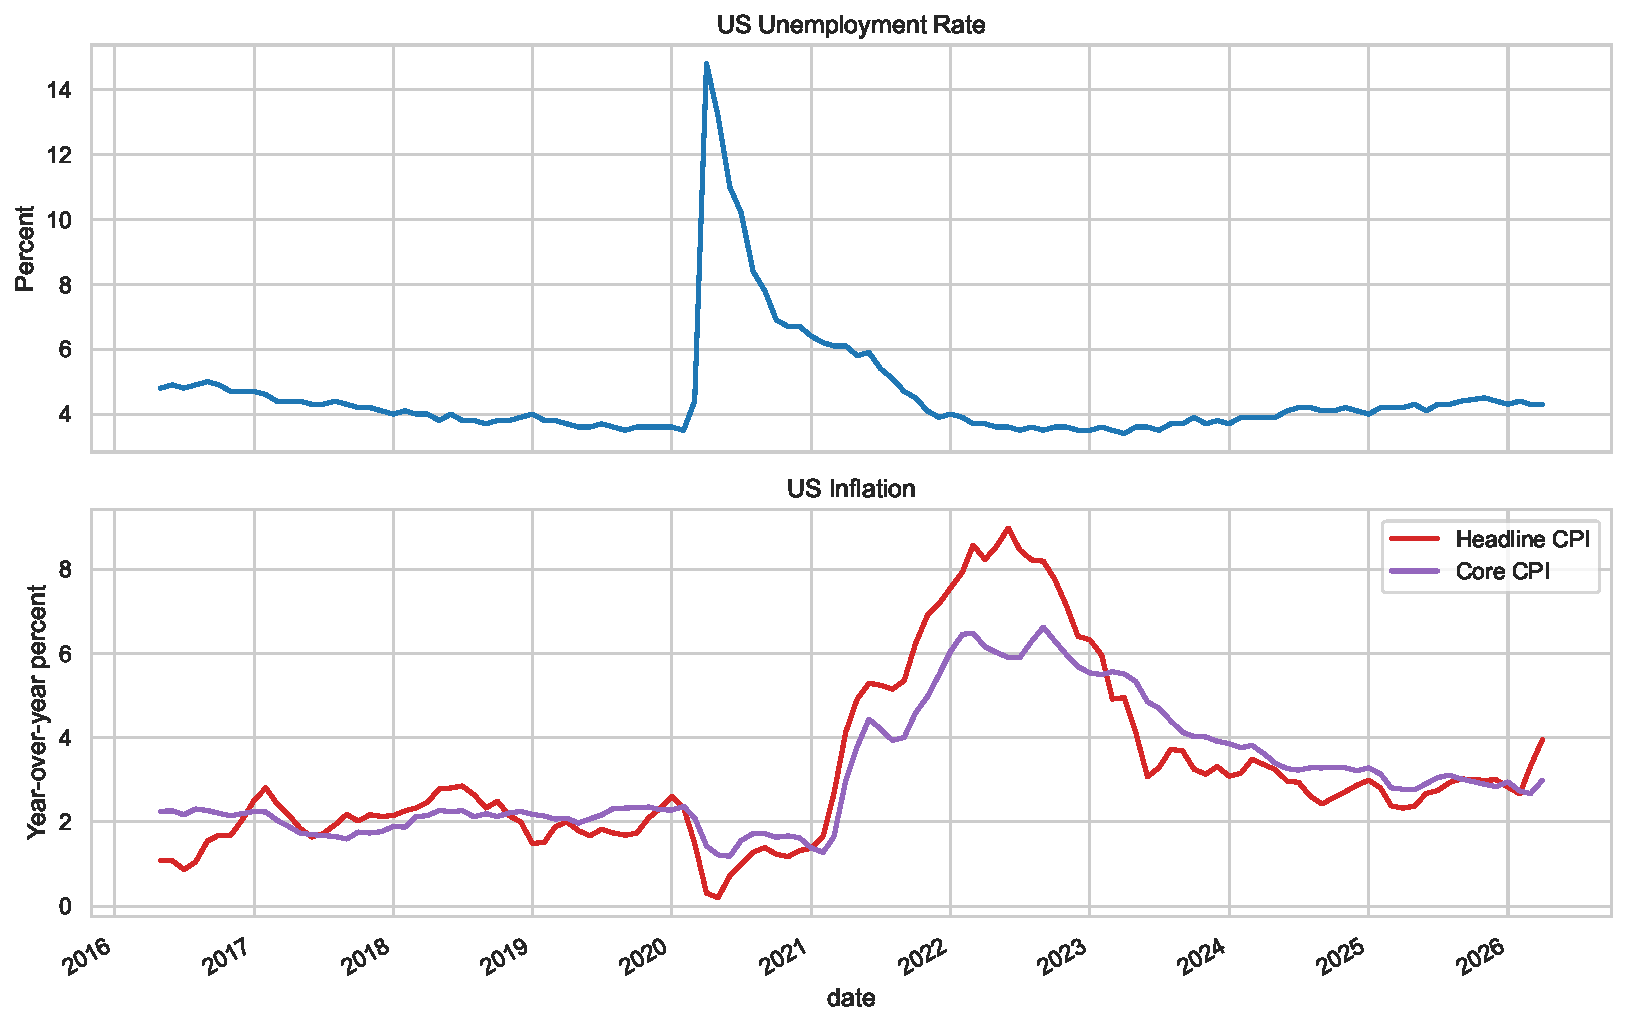
\includegraphics[width=0.95\textwidth]{report_assets/labor_inflation.pdf}
    \caption{Unemployment, headline inflation, and core inflation.}
\end{figure}

\section*{How Inflation and Unemployment Interacted}
The traditional Phillips curve says that inflation should rise when unemployment is low, because a tight labor market can increase wage and price pressures. In practice, the relationship may be curved rather than a straight line. We therefore compare a linear fit with a quadratic fit, which allows the relationship to bend when the labor market is very tight or very weak.

\begin{figure}[H]
    \centering
    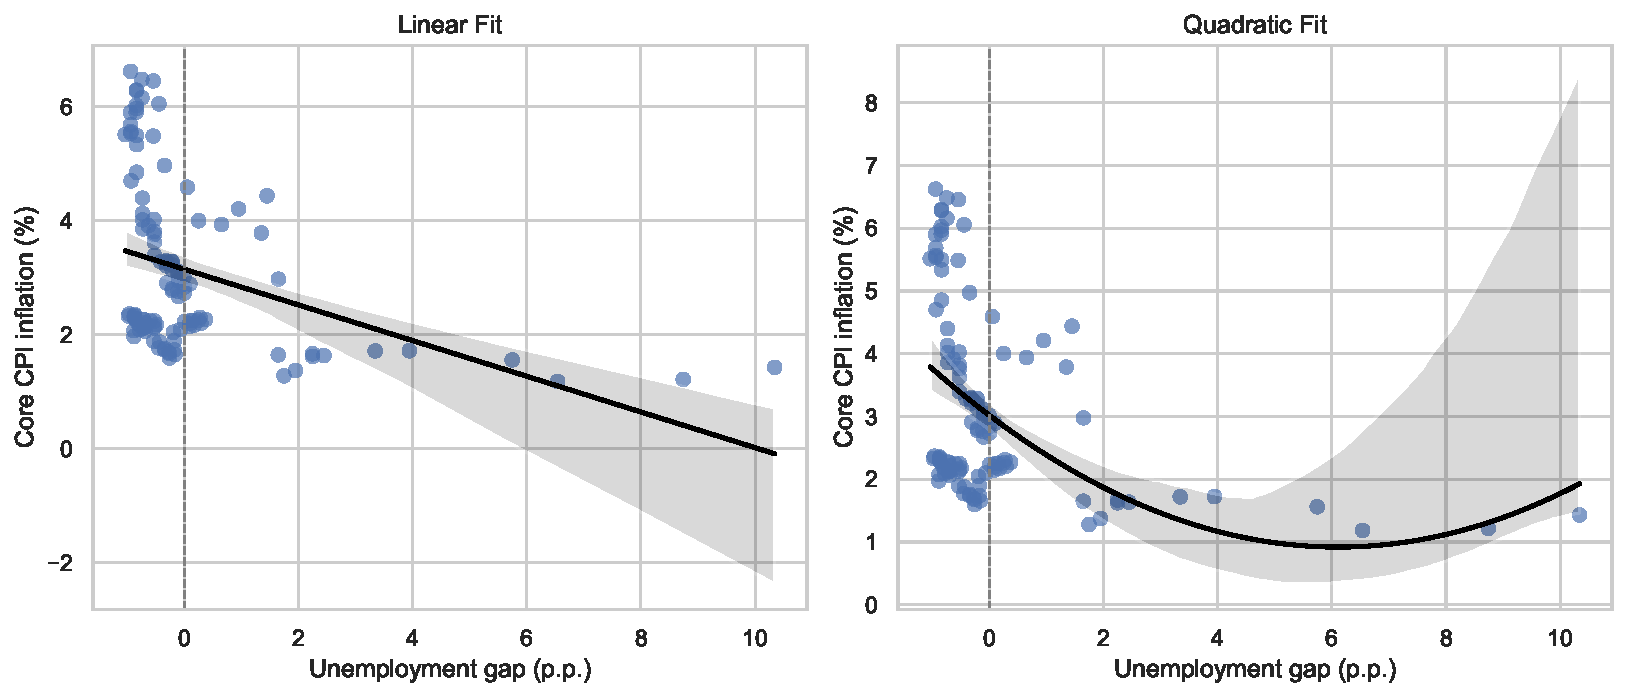
\includegraphics[width=0.95\textwidth]{report_assets/phillips_scatter.pdf}
    \caption{Phillips curve views: linear and quadratic fits using the unemployment gap.}
\end{figure}

\section*{Model Results}
We estimated four simple models. The final specification uses core inflation, the unemployment gap, the square of the unemployment gap, and lagged core inflation. The squared term allows for a curved Phillips curve. Lagged inflation is included because inflation is usually persistent: this month's inflation is strongly related to recent inflation.

\begin{table}[H]
\centering
\small
\begin{tabular}{p{2.8cm}p{3.0cm}p{3.1cm}rrr}
\toprule
Model & Dependent variable & Labor-market variable & Coef. & p-value & R$^2$ \\
\midrule
Simple model & Headline inflation & Unemployment rate & -0.430 & 0.008 & 0.130 \\
Gap model & Headline inflation & Unemployment gap & -0.414 & 0.007 & 0.120 \\
Augmented linear & Core inflation & Unemployment gap & -0.011 & 0.599 & 0.972 \\
Augmented quadratic & Core inflation & Gap + gap squared & 0.097 & 0.011 & 0.975 \\
\bottomrule
\end{tabular}
\caption{Phillips curve model comparison. Standard errors use a HAC correction.}
\end{table}

In the augmented linear model, the unemployment-gap coefficient is -0.0108 with a p-value of 0.5993. This means the estimated relationship is negative, as the traditional Phillips curve would suggest, but it is not statistically strong in this recent 10-year sample.

The quadratic model changes the interpretation. The coefficient on the unemployment gap is 0.0972, and the coefficient on the squared unemployment gap is -0.0153. The squared term has a p-value of 0.0005. At the latest unemployment gap, the model-implied association is that a 1 percentage point higher unemployment gap is linked to about 0.100 percentage points higher core inflation, holding lagged inflation constant. Around a normal labor market, where the unemployment gap is zero, the model-implied association is about 0.097 percentage points higher. This shows why the quadratic form should be read carefully: the implied effect is not constant across the cycle.

The lagged core inflation coefficient is 0.9994 with a p-value of 0.0000. This indicates strong inflation persistence. In practical terms, recent inflation explains current inflation better than unemployment does in this sample.

When the COVID period is excluded, the unemployment-gap coefficient is -0.0204 with a p-value of 0.7994. This check helps show whether the pandemic period is driving the conclusion.

\section*{Causality and Practical Meaning}
These regressions should be read as associations, not proof of causality. For example, the model can say that a 1 percentage point higher unemployment gap is associated with a certain change in inflation, holding other included variables constant. This is different from saying that unemployment mechanically caused inflation to fall by that amount. Also note the unit: unemployment rates move in percentage points, so a move from 4\% to 5\% unemployment is a 1 percentage point increase.

We also ran a Granger-causality check with up to six monthly lags. This test asks whether past unemployment gaps help predict current core inflation, and whether past core inflation helps predict the unemployment gap. The best p-value for unemployment helping predict inflation was 0.2999. The best p-value for inflation helping predict unemployment was 0.2240. Since both are above 0.05, the test does not provide strong evidence of predictive causality in either direction. This is a forecasting test, not proof of economic causality.

\section*{Client-Friendly Interpretation}
The recent US Phillips curve is not absent, but it is weak. Allowing the curve to bend adds flexibility, but it does not overturn the main conclusion: low unemployment alone did not explain the inflation surge of 2021--2023. A more complete explanation needs inflation persistence, pandemic disruptions, supply conditions, energy prices, and expectations.

For investors and bank clients, the main message is that inflation risk should not be judged only by the unemployment rate. Labor-market tightness matters, but recent inflation dynamics show that price pressures can remain elevated even when the direct unemployment-inflation relationship is statistically modest.

\section*{Data Source}
Data are from the Federal Reserve Bank of St. Louis FRED database: UNRATE, CPIAUCSL, CPILFESL, and NROU. Inflation rates are calculated as year-over-year percentage changes.

\end{document}
